\chapter{Introduction to Bessel Functions}\label{lec:lec43}
So far we have treated the rectangular waveguide. In this chapter, we will be discussing the circular waveguide. It is a waveguide with a circular cross-section in the transverse plane whose wave propagates in the z-direction. It has metallic walls like a metal pipe and we will understand how waves propagate in this guide. It is useful for making quality \emph{cavity resonators}\index{cavity resonator}\textemdash\;a structure used to store energy. To solve the problem of how the wave propagates in a circular waveguide, we will use the cylindrical coordinates system.

Now the Helmholtz\footnote{
Hermann Ludwig Ferdinand Von Helmholtz (31/08/1821\textemdash08/09/1894) was a German physician and physicist who made significant contributions to several scientific fields.  The Helmholtz equation is typically expressed as:
\begin{align*}    
\nabla^2\Psi + k^2\Psi = 0
\end{align*}
where $\nabla^2$ is the Laplacian operator, $\Psi$ represents the unknown function, $k$ is the wave number, and the equation holds in three-dimensional space. The Helmholtz equation arises when studying the behaviour of waves in different physical systems and is an essential tool for solving wave equations and understanding wave phenomena
} wave equation:
\begin{align}
\nabla^2 \bar{E} + h^2 \bar{E} = 0\label{eqn:helmholtzelectric}\\
\nabla^2 \bar{H} + h^2 \bar{H} = 0\label{eqn:helmholtzmagnetic}
\end{align}
Considering the electric field component, $E_z$, Equation~\eqref{eqn:helmholtzelectric} becomes:
\begin{align*}
\frac{1}{r} \partialderivative{}{r}\partialderivative{E_z}{r} + \frac{1}{r^2} \partialderivative[2]{E_z}{\phi} + h^2 E_z = 0
\end{align*}
Where $h^2 = \omega^2 \mu \epsilon + \gamma^2$ and the solution of this partial differential equation (PDE)\index{partial differential equation} is the \emph{Bessel function}\index{bessel function}. Therefore in this section, we will introduce the Bessel function.

\section{Bessel Function}
Consider the second-order ordinary differential equation (ODE) given as follows:
\begin{align}
x^2 \derivative[2]{y}{x} + x \derivative{y}{x} + (x^2 - n^2)y = 0
\label{eqn:secondorderode}
\end{align}
The first solution to Equation~\eqref{eqn:secondorderode} was proposed by Daniel Bernoulli,\footnote{
Daniel Bernoulli (8/02/1700\textemdash17/03/1782) was a Swiss mathematician and physicist and was one of many prominent mathematicians in the Bernoulli family. He is particularly remembered for his applications of mathematics to mechanics, especially fluid mechanics, and his pioneering work in probability and statistics. His name is commemorated in Bernoulli's principle, a particular example of the conservation of energy, which describes the mathematics of mechanism underlying the operation of two important technologies of the 20th century: the carburettor and the aeroplane wing.
}
from the famous Bernoulli principle and it was for analysis of a hanging chain (how it oscillates). We all know a pendulum and therefore we have studied its oscillation with a fixed length of chain. However, there is an oscillation when the length is not fixed and that oscillation was described by Daniel Bernoulli. The second solution was by L. Euler\footnote{
Leonard Euler (15/04/1707\textemdash18/09/1783) was a Swiss mathematician, physicist, astronomer, logician, and engineer, who made important and influential discoveries in many branches of mathematics, such as infinitesimal calculus and graph theory, while also making pioneering contributions to several branches such as topology and analytic number theory. He also introduced much of the modern mathematical terminology and notation, particularly for mathematical analysis, such as the notion of a mathematical function.
} famous for the Euler formula and it was for the theory of vibrations of a circular membrane. For instance, the vibrations on a circular drum. In the end, it was Friedrich Bessel\footnote{
Friedrich Wilhelm Bessel (22/7/784\textemdash17/03/1846) German Astronomer, mathematician, physicist and geodesist, influenced by Carl Friedrich Wihhelm Argelander. Laplace function was named after him in his death even if originally discovered by Daniel Bernoulli.
} who did a systematic study of the PDE and proposed the various forms of the solution which form the basis of the Bessel function and Equation~\eqref{eqn:secondorderode} is called the \emph{Bessel equation}. Bessel functions are probably the next important functions to sines and cosines functions. They play a role in electromagnetics, heat transfer, wave motion, elasticity, and scattering problems\textemdash where waves are scattered from a cylinder or fluids are scattered in a microfluidic channel with cylindrical dimensions. Essentially, any time there is a cylindrical symmetry, the solution is a Bessel function.

From Equation~\eqref{eqn:secondorderode}, the symbol n is a real number which is positive or zero. Let us denote $\derivative[2]{y}{x} \equiv y''$ and $\derivative{y}{x} \equiv y'$, so that
\begin{align*}
x^2y'' + xy' + (x^2 - n^2)y = 0
\end{align*}
\begin{equation}
x(xy')' + (x^2 - n^2)y = 0
\label{eqn:secondorderode2}
\end{equation} 
For a second-order PDE, we use the series expansion as the solution of the equation which is the Frobenius method\footnote{
Ferdinand George Frobenius  (26/10/1849\textemdash03/08/1971) was a German mathematician, best known for his contributions to the theory of elliptic functions, differential equations, number theory, and to group theory. He is known for the famous determinantal identities, known as Frobenius- Stickelberger formulae, governing elliptic functions, and for developing the theory of biquadratic forms.
}. So, the proposed solution is 
\begin{align}
y(x) = \sum_{k=0}^{\infty}C_k x^{k + \alpha}
\label{eqn:besselfunctionsoln}
\end{align}
which is a general power series solution where $\alpha$ is a constant we introduce to the power of x since the power of x may not necessarily be an integer. Now let us take the derivative of the proposed solution and substitute for the terms $x(xy')'$ and y in Equation~\eqref{eqn:secondorderode2}.
\begin{align*}
y' &= \sum_{k=0}^{\infty}C_k (k + \alpha) x^{k + \alpha - 1}\\
xy' &= \sum_{k=0}^{\infty}C_k (k + \alpha) x^{k + \alpha}\\
(xy')' &= \sum_{k=0}^{\infty}C_k (k + \alpha)^2 x^{k + \alpha - 1}\\
x(xy')' &= \sum_{k=0}^{\infty}C_k (k + \alpha)^2 x^{k + \alpha}
\end{align*}
Substituting the above terms in Equation~\eqref{eqn:secondorderode2} we get
\begin{align*}
\sum_{k=0}^{\infty}C_k (k + \alpha)^2 x^{k + \alpha} + (x^2 - n^2)\sum_{k=0}^{\infty}C_k x^{k + \alpha} = 0
\end{align*}
\begin{dmath}
\sum_{k=0}^{\infty}C_k (k + \alpha)^2 x^{k + \alpha} - n^2\sum_{k=0}^{\infty}C_k x^{k + \alpha} + \sum_{k=0}^{\infty}C_k x^{k + \alpha + 2} = 0
\label{eqn:secondorderode3}
\end{dmath}
Now we need to determine the various coefficient $C_k$ and the term $\alpha$ we have introduced. The values will be determined by the equation above. First, we note that the equation is true for all powers of x i.e. for $x^0, x^1, x^2$ and so on, hence we have a combination of infinite equations. So let us consider Equation~\eqref{eqn:secondorderode3} for $k=0$, we have 
\[
C_0 \alpha^2 x^\alpha - n^2C_0 x^\alpha + C_0 x^{\alpha + 2} =0
\]
Considering similar exponents of x gives 
\begin{align*}
C_0 \alpha^2 x^\alpha - n^2C_0 x^\alpha &=0\\
C_0 x^\alpha(\alpha^2 -n^2) &=0
\end{align*}
Therefore, $C_0 =0$ or $(\alpha^2 -n^2) =0$. $C_0 =0$ makes no sense, it means the solution is not going to exist so  $\alpha^2 -n^2 =0$ or  $\alpha =\pm n$. Now let us consider the coefficients of $x^{\alpha + 1}$ for $k=1$ in Equation~\eqref{eqn:secondorderode3}.
\begin{align*}
C_1(1 + \alpha)^2 x^{1 + \alpha} - n^2 C_1 x^{1 + \alpha} &= 0\\
C_1x^{1 + \alpha}[(1 + \alpha)^2 - n^2] &= 0\\
C_1x^{1 + \alpha}[1 + \alpha^2 + 2\alpha - n^2] &=0\quad\text{Since }\alpha^2 = n^2\\
C_1x^{1 + \alpha}[1 + 2\alpha] &=0\quad\text{For }\alpha =\pm n\\
C_1x^{1 + \alpha}[1 + 2(\pm n)] &= 0
\end{align*}
This means that $C_1 = 0$, since $n \geqq 0$. Now let us consider the coefficients of $x^{\alpha + 2}$ for $k=2$ and $k=0$ in Equation~\eqref{eqn:secondorderode3}.
So 
\begin{align*}
C_2(2 + \alpha) x^{2 + \alpha} - n^2 C_2x^{2 + \alpha} + C_0x^{2 + \alpha} = 0\\
C_0 = C_2[n^2 - (2 + \alpha)^2]
\end{align*}
We can generalize this relationship since a coefficient is always related to 2 coefficients behind, therefore,
\begin{dmath}
C_{k-2} = C_k (n^2 - (k + \alpha)^2)\quad\text{or}\\
C_k\text{ = }\frac{C_{k-2}}{[n^2 - (k + \alpha)^2]}
\label{eqn:coefficients}
\end{dmath}
If k is odd for instance $k = 3$, then Equation~\eqref{eqn:coefficients} becomes
\begin{align*}
C_3 = \frac{C_{1}}{n^2 - (3 + \alpha)^2} = 0\quad\text{since }C_1 = 0
\end{align*} 

Also, $C_5$ will be related to $C_3$ and so the odd coefficient does not exist while for even values of k, there are even coefficients. Let $\alpha = \pm n$, so Equation~\eqref{eqn:coefficients} becomes 
\begin{dmath*}
C_k = \frac{C_{k-2}}{n^2 - (k + n)^2} 
= \frac{C_{k-2}}{n^2 - k^2 - n^2 - 2nk}
=\frac{(-1) C_{k-2}}{k^2 + 2nk} 
= \frac{(-1) C_{k-2}}{k(2n + k)}\quad\text{where k is even.}
\end{dmath*} 
Let $k =2k$, such that $k = 1, 2, 3, \ldots$.
\begin{dmath}
C_{2k} = \frac{(-1) C_{2k-2}}{2k(2n + 2k)} 
= \frac{(-1) C_{2k-2}}{4k(n + k)}
\label{eqn:coefficients2}  
\end{dmath}
For $k=1$
\[
C_2 = \frac{(-1) C_0}{4(n + 1)} = \frac{(-1) C_0}{2^2(n + 1)}
\]
For $k = 2$
\begin{align*}
C_4 =& \frac{(-1) C_2}{2^2 2(2 + n)}\quad\text{substituting }C_2\\
=& \frac{(-1)^2 C_0}{2^4 2(n + 2)(n + 1)}
\end{align*}
There seems to be a pattern and to find it let us find one more term so we can get a generalized relationship.

For $k = 3$
\begin{dmath*}
C_6 = \frac{(-1) C_4}{2^2 3(n + 3)}
= \frac{(-1)^3 C_0}{2^6 3!(n + 3)(n + 2)(n + 1)}
\end{dmath*}
Hence, the general expression is as follows:
\begin{equation} 
C_{2k} = \frac{(-1)^k C_0}{2^{2k} k!(n + k)(n + k-1)\ldots(n + 1)}
\end{equation}
Let us introduce the Gamma functions, $\Gamma(\cdot)$, to simplify the expression a little further. The \emph{Gamma function}\index{gamma function} is factorial but unlike factorial which works for only integers, it can be done with any number so it is a generalized factorial function. It is given as 
\[
\Gamma(n + 1) = n \Gamma(n)
\]
So for $n = n + 1$, the Gamma function will be given as
\[
\Gamma(n + 2) = (n + 1)\Gamma(n + 1)
\]
The same applies to higher values of n i.e. 
\begin{align*}
\Gamma(n + 3) &= (n + 2)\Gamma(n + 2)\quad\text{substituting }\Gamma(n + 2)\\
&= (n + 2)(n + 1)\Gamma(n + 1)\quad\text{and so on.}
\end{align*}

Let us rewrite the expression for $C_{2k}$ in terms of the Gamma function, but first considering $C_2$, we have
\begin{align*}
C_2 =& \frac{(-1)^1 C_0}{2^2(n + 1)}\quad\text{substituting }n + 1 = \frac{\Gamma(n + 1)}{\Gamma(n + 2)}\\
=& \frac{(-1)^1 C_0 \Gamma(n + 1)}{2^2 \Gamma(n + 2)}
\end{align*}
So the generalized relationship is 
\begin{equation}
C_{2k} =  \frac{(-1)^k C_0 \Gamma(n + 1)}{2^{2k} k! \Gamma(n + k + 1)}
\label{eqn:coefficients3}
\end{equation}

At this point, we have the series solution for the Bessel equation where $\alpha= +n$ as 
\begin{dmath}
y(x) = C_0 x^n \Gamma(n + 1) \left\lbrace\frac{1}{\Gamma(n + 1)} - \frac{1}{\Gamma(n+2)}\left(\frac{x}{2}\right)^2 +\frac{1}{2!\Gamma(n+3)}\left(\frac{x}{2}\right)^4 - \frac{1}{3!\Gamma(n+4)}\left(\frac{x}{2}\right)^6 + \ldots \right\rbrace\quad\text{let }C_0\text{ = }\frac{1}{2^n \Gamma(n + 1)}
= \left(\frac{x}{2}\right)^n \left\lbrace\frac{1}{\Gamma(n + 1)} - \frac{1}{\Gamma(n+2)}\left(\frac{x}{2}\right)^2 +\frac{1}{2!\Gamma(n+3)}\left(\frac{x}{2}\right)^4 - \frac{1}{3!\Gamma(n+4)}\left(\frac{x}{2}\right)^6 + \ldots\right\rbrace
\label{eqn:besselsolnseries}
\end{dmath}
Equation~\eqref{eqn:besselsolnseries} is called the \emph{Bessel function\index{bessel function} of the first kind}. The function has an order of n and it is represented by the term $J_n(x)$
where J is the Bessel function of the first kind, n is the order and x is the variable. It can be rewritten as 
\begin{equation}
J_n(x) = \sum_{k = 0}^{\infty}\frac{(-1)^k (\frac{x}{2})^{2k + n}}{k! \Gamma(n + k + 1)}
\label{eqn:besselsolnseries2}
\end{equation}

Using Equation~\eqref{eqn:besselsolnseries2}, let us consider the Bessel function for the zeroth order i.e. $n=0$
\begin{align*}
J_0(x) = 1 - \frac{(\frac{x}{2})^2 }{1!} + \frac{(\frac{x}{2})^4 }{(2!)^2} - \frac{(\frac{x}{2})^6 }{(3!)^2} + \ldots
\end{align*}
if $\alpha = -n,$ then,
\begin{equation}
J_{-n}(x) = \sum_{k = 0}^{\infty}\frac{(-1)^k (\frac{x}{2})^{2k - n}}{k! \Gamma(-n + k + 1)}
\label{eqn:besselsolnseries3}
\end{equation}
In general, we would expect the solution of the Bessel equation as 
\[
y(x) = A J_n(x) + B J_{-n} (x)
\]
However, this solution is only true if n is not an integer. This is because when n is an integer the two terms are linearly dependent, and are related by $ J_{-n}(x) = (-1)^n J_n(x)$ which shows $J_{-n}(x)$ is linearly related to $ J_n(x).$ This can be shown by referring once again to our knowledge of gamma functions.

We know that $\Gamma(n + 1) = n \Gamma(n)$, so 	$\Gamma(n) = \frac{\Gamma(n + 1)}{n} $ and for negative integer values of n, or zero, $\Gamma(n)$ is infinite. So from Equation~\ref{eqn:besselsolnseries3}, the coefficients of the first n terms become zero since the gamma function is infinite and the summation starts with $k=n$, thus
\begin{align*}
J_n(x) &= \sum_{k = n}^{\infty}\frac{(-1)^k (\frac{x}{2})^{2k - n}}{k! \Gamma(-n + k + 1)}\quad\text{substituting }m\text{ = }k - n\\
J_{-n}(x) &= \sum_{m = 0}^{\infty}\frac{(-1)^{m + n} (\frac{x}{2})^{2m + n}}{(m + n)! \Gamma(m + 1)}\\
&= \sum_{m = 0}^{\infty}\frac{(-1)^{m + n} (\frac{x}{2})^{2m + n}}{(m + n)! m!}\footnotemark
\end{align*}
\footnotetext{
m is an integer
}
Comparing this result with
\[
J_n(x) = \sum_{k = 0}^{\infty}\frac{(-1)^k (\frac{x}{2})^{2k + n}}{(k + n)! k!}
\]
Where $\Gamma(n + k - 1)=(n + k)!$ for $n= integer$, we see that
\begin{equation}
J_{-n}(x) = (-1)^n J_n(x)
\label{eqn:besselsolnseries4}
\end{equation}
In electromagnetics and optics, n is an integer hence $J_{-n}$ is not an independent solution. Now let us physically examine the function $J_n(x)$. Consider a specific case of $n = \frac{-1}{2}$
\begin{align*}
J_{-\frac{1}{2}}(x) &= \sum_{k = 0}^{\infty}\frac{(-1)^k (\frac{x}{2})^{2k - \frac{1}{2}}}{k! \Gamma( k + \frac{1}{2})}\\&\text{where }\Gamma\left( k + \frac{1}{2}\right)\text{ = }\frac{(2k - 1)! \sqrt{\pi}}{2^{2k - 1}(k - 1)!}\text{ and }\Gamma\left(\frac{1}{2}\right)\text{ = }\sqrt{\pi}\\
&= \sqrt{\frac{2}{\pi x}}\sum_{k = 0}^{\infty}\frac{(-1)^k x^{2k}}{(2k!)}\\&\text{where }\cos x\text{ = }\sum_{k = 0}^{\infty}\frac{(-1)^k x^2k}{(2k!)}\\
&= \sqrt{\frac{2}{\pi}}\frac{1}{\sqrt{x}}\cos(x)
\end{align*}
Similarly for $n = \frac{1}{2}$
\begin{align*}
J_{\frac{1}{2}}(x) = \sqrt{\frac{2}{\pi}}\frac{1}{\sqrt{x}}\sin(x)
\end{align*}

Figure~\ref{fig:fig-1} shows the plot of the Bessel function, $ J_{-\frac{1}{2}}(x)$.
\begin{figure}[h]
\centering
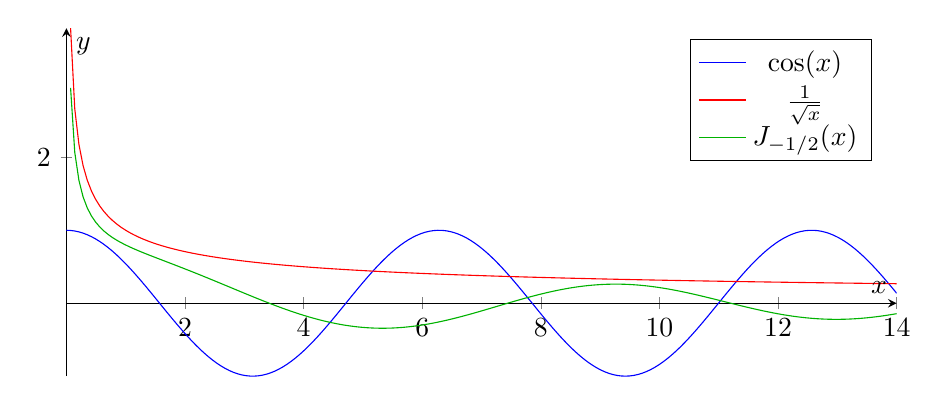
\begin{tikzpicture}
\begin{axis}[
    xlabel=$x$,
    ylabel=$y$,
    domain=0:14,
    samples=200,
    legend pos=north east,
    axis lines=middle,
    width=1\linewidth,
    height=6cm,
]

% Cosine function
\addplot [blue] {cos(deg(x))};
\addlegendentry{$\cos(x)$};

% 1/sqrt(x) function
\addplot [red] {1/sqrt(x)};
\addlegendentry{$\frac{1}{\sqrt{x}}$};

% Bessel function
\addplot [green!70!black] {sqrt(2/(pi*x))*cos(deg(x-sqrt(x)))};
\addlegendentry{$J_{-1/2}(x)$};

\end{axis}
\end{tikzpicture}
\caption{Plot of $\cos(x)$, $\frac{1}{\sqrt{x}}$, and $J_{-1/2}(x)$}
\label{fig:fig-1}
\end{figure}

It shows the Bessel function,$J_{-\frac{1}{2}}$ , is the product of $\frac{1}{\sqrt{x}}$ and $\cos(x)$ which are plotted differently. It is seen that at $x=0$, $\frac{1}{\sqrt{x}}$ goes to infinity and as x increases the $\frac{1}{\sqrt{x}}$ term decreases rapidly as shown. The product of the two functions $(\cos(x)$ and $\frac{1}{\sqrt{x}}$) gives the resulting plot of $J_{-\frac{1}{2}}(x)$. It is seen that the zero points are maintained so $J_{-\frac{1}{2}}(x)$ has the periodicity of $\cos(x)$ but the lobes or amplitude of $J_{-\frac{1}{2}}(x)$ goes on decreasing in value as x increases. Let us see some more plots of the Bessel functions, $J_n(x)$ for different values of n. Figure~\ref{fig:bessel-functions} shows the plot of Bessel functions of positive order $J_{n}(x)$.
\begin{figure}[h]
\centering
\includegraphics[width=1\linewidth]{/graphics/BesselJ_800}
\caption{Plot of Bessel functions of positive order $J_{n}(x)$}
\label{fig:bessel-functions}
\end{figure}

We will proceed to consider the \emph{Bessel function of the second kind} also called the \emph{Neumann function}\index{neumann function} as a second solution to the Bessel equation when n is an integer. It is given by: 
\begin{align}
Y_n = \frac{\cos(n\pi) J_n(x) - J_{-n}(x)}{\sin(n\pi)}
\label{eqn:neumannfunctions}
\end{align}
As we have seen from the plot of $J_n(x)$ that every Bessel function of the first kind has a zero value at the centre i.e at $x= 0$ except for $J_-{\frac{1}{2}}(x)$ and $J_0(x)$, where $J_0(x)$ has a peak value at $ x= 0$. Suppose we want to confine the wave such that it is within a single lobe of the function then the solution is of the order of $n =0$ which is $J_0(x)$. On the other hand, the Neumann functions always start from $-\infty$ at $x=0$ (centre of the waveguide) as shown in Figure~\ref{fig:fig-3}.
\begin{figure}[h]
\centering
\includegraphics[width=1\linewidth]{/graphics/BesselY_800}
\caption{ Plot of the Neumann functions}
\label{fig:fig-3}
\end{figure}

In general, we will have a solution of the form if n is an integer
\begin{equation*}
y(x) = AJ_n(x) + B Y_n(x)\quad\text{where A and B are constants.}
\end{equation*}
In reality, since $Y_n(0) = -\infty$, it makes no physical sense in electromagnetics and electrodynamics so the solution will be 
\begin{equation}
y(x) = AJ_n(x)
\end{equation}
This concludes the discussion on Bessel functions and next, we will discuss circular waveguides. So in this chapter, we looked at a general introduction to Bessel functions and as electrical engineers, these functions play a very important role in cylindrical symmetry. For the circular waveguide which we will discuss in the next chapter, the Bessel function of the first kind is important in its analysis. Another area of waveguide that concerns itself with Bessel functions is dielectric waveguides such as the optical fibre. In their analysis, we consider the function called the \emph{Hankel function}\footnote{
Hermann Hankel(14/02/1839\textemdash29/08/1873), was a German mathematician, known for his contributions to mathematics, specifically in the field of special functions. He developed the Henkel function, also known as the Hermann Henkel function, which is a solution to a certain class of ordinary differential equations. Henkel's work on the Henkel function has found applications in various areas of physics, engineering, and mathematical analysis. His contributions have had a significant impact on the understanding and utilization of special functions in mathematical research and practical applications.
}\index{henkel function} which is the \emph{Bessel function of the third kind}. It is basically an exponentially decaying function equivalent to the $e^{-\alpha x}$ kind of function for the dielectric waveguide.
